%%
%%   This file is part of ICTP RegCM.
%%
%%   ICTP RegCM is free software: you can redistribute it and/or modify
%%   it under the terms of the GNU General Public License as published by
%%   the Free Software Foundation, either version 3 of the License, or
%%   (at your option) any later version.
%%
%%   ICTP RegCM is distributed in the hope that it will be useful,
%%   but WITHOUT ANY WARRANTY; without even the implied warranty of
%%   MERCHANTABILITY or FITNESS FOR A PARTICULAR PURPOSE.  See the
%%   GNU General Public License for more details.
%%
%%   You should have received a copy of the GNU General Public License
%%   along with ICTP RegCM.  If not, see <http://www.gnu.org/licenses/>.
%%

\chapter{Description}

\section{History}

The idea that \ac{LAMs} could be used for regional studies was originally
proposed by \citet{Dickinson_89} and \citet{Giorgi_90}.

It was based on the concept of one-way nesting, in which large scale
meteorological fields from \ac{GCM} runs provide initial and time-dependent
meteorological \ac{LBCs} for high resolution \ac{RCM} simulations, with no
feedback from the \ac{RCM} to the driving \ac{GCM}.

The first generation NCAR \ac{RegCM} was built upon the \ac{NCAR}-\ac{PSU}
\ac{MM4} in the late 1980s \citep{Dickinson_89, Giorgi_89}. The dynamical
component of the model originated from the \ac{MM4}, which is a compressible,
finite difference model with hydrostatic balance and vertical
$\sigma$-coordinates.

Later, the use of a split-explicit time integration scheme was added along
with an algorithm for reducing horizontal diffusion in the presence of steep
topographical gradients \citep{Giorgi_93,Giorgi_93b}.

As a result, the dynamical core of the \ac{RegCM} is similar to that of the
hydrostatic version of \ac{MM5} \citep{Grell_94}: the \ac{RegCM}4 
hydrostatic is thus a compressible, sigma-p vertical coordinate model run on an
Arakawa B-grid in which wind and thermodynamical variables are horizontally
staggered using a time-splitting explicit integration scheme in which the two
fastest gravity modes are first separated from the model solution and then
integrated with smaller time steps.

For application of the \ac{MM4} to climate studies, a number of physics
parameterizations were replaced, mostly in the areas of radiative transfer and
land surface physics, which led to the first generation \ac{RegCM}
\citep{Dickinson_89,Giorgi_90}. The first generation \ac{RegCM} included the
Biosphere-Atmosphere Transfer Scheme, BATS, \citep{Dickinson_86} for surface
process representation, the radiative transfer scheme of the \ac{CCM1}, a medium
resolution local planetary boundary layer scheme, the Kuo-type cumulus
convection scheme of \citep{Anthes_77} and the explicit moisture scheme of
\citep{Hsie_84}.

A first major upgrade of the model physics and numerical schemes was documented
by \citep{Giorgi_93,Giorgi_93b}, and resulted in a second generation \ac{RegCM},
hereafter referred to as \ac{RegCM2}. The physics of \ac{RegCM2} was based on
that of the \ac{NCAR} \ac{CCM2} \citep{Hack_93}, and the mesoscale model
\ac{MM5} \citep{Grell_94}. In particular, the \ac{CCM2} radiative transfer
package \citep{Briegleb_92} was used for radiation calculations, the non local
boundary layer scheme of \citep{Holtslag_90} replaced the older local scheme,
the mass flux cumulus cloud scheme of \citep{Grell_93} was added as an option,
and the latest version of BATS1E \citep{Dickinson_93} was included in the model.

In the last few years, some new physics schemes have become available for use in
the \ac{RegCM}, mostly based on physics schemes of the latest version of the
\ac{CCM}, \ac{CCM3} \citep{Kiehl_96}. First, the \ac{CCM2} radiative transfer
package has been replaced by that of the \ac{CCM3}. In the \ac{CCM2} package,
the effects of ${\rm H_2O}$, ${\rm O_3}$, ${\rm O_2}$, ${\rm CO_2}$ and clouds
were accounted for by the model. Solar radiative transfer was treated with a
$\delta$-Eddington approach and cloud radiation depended on three cloud
parameters, the cloud fractional cover, the cloud liquid water content, and the
cloud effective droplet radius. The \ac{CCM3} scheme retains the same structure
as that of the \ac{CCM2}, but it includes new features such as the effect of
additional greenhouse gases (${\rm NO_2, CH_4, CFCs}$), atmospheric aerosols,
and cloud ice. Scattering and absorption of solar radiation by aerosols are
also included based on the aerosol optical properties (Absorption Coefficient
and Single Scattering Albedo).
 
A simplified explicit moisture scheme \citet{Hsie_84} is included, where only a
prognostic equation for cloud water is used, which accounts for cloud water
formation, advection and mixing by turbulence, re-evaporation in sub-saturated
conditions, and conversion into rain via a bulk autoconversion term.
Prognosed cloud water variable is directly used in the cloud
radiation calculations, and not diagnosed in terms of the local
relative humidity, adding a very important and far reaching element of
interaction between the simulated hydrologic cycle and energy budget
calculations. 

The solar spectrum optical properties are based on the cloud liquid water path,
which is in turn based on the cloud liquid water amount prognostically
calculated by the model, cloud fractional cover, which is calculated
diagnostically as a function of relative humidity, and effective cloud droplet
radius, which is parameterized as a function of temperature and land sea mask
for liquid water and as a function of height for ice phase.

In addition, the scheme diagnostically calculates a fraction of cloud ice as a
function of temperature. In the infrared spectrum the cloud emissivity is
calculated as a function of cloud liquid/ice water path and cloud infrared
absorption cross sections depending on effective radii for the liquid and ice
phase.

One of the problems in this formulation is that the scheme uses the cloud
fractional cover to produce grid box mean cloud properties which are then
treated as if the entire grid box was covered by an effectively thinner
cloud layer. However, because of the non-linear nature of radiative transfer,
this approach tends to produce a grayer mean grid box than if separate
cloudy and clear sky fractional fluxes were calculated. By taking advantage
of the fact that the scheme also calculates clear sky fluxes for diagnostic
purposes, in \ac{RegCM}4 we modified this radiative cloud representation by
first calculating the total cloud cover at a given grid point and then
calculating the surface fluxes separately for the cloudy and clear sky
portions of the grid box.

The total cloud cover at a model grid box is given by a value
intermediate between that obtained using the random overlap assumption
(which maximizes cloud cover) and that given by the largest cloud cover
found in any single layer of the column overlying the grid box (which implies
a full overlap and it is thus is a minimum estimate of total cloud cover).

This modification thus accounts for the occurrence of fractional clear sky at
a given grid box, leading to more realistic grid-box average surface radiative
fluxes in fractional cloudy conditions.

A large-scale cloud and precipitation scheme which accounts for the
subgrid-scale variability of clouds \citep{Pal_00}, parameterizations for
ocean surface fluxes \citep{Zeng_98}, and multiple cumulus convection scheme
\citep{Anthes_77,Grell_93,Emanuel_91,Emanuel_99} are the same as in \ac{RegCM}3,
but a new "mixed scheme" Grell+Emanuel is introduced: it allows the user to
select one of the two schemes in function of the ocean-land mask.

The other main development compared to \ac{RegCM}3 concerns the aerosol
radiative transfer calculations. In \ac{RegCM}3 the aerosol radiative forcing
was based on three dimensional fields produced by the aerosol model, and
included only scattering and absorption in the shortwave spectrum (see
\cite{Giorgi_02}). In \ac{RegCM}4 we added the contribution of the infrared
spectrum following \cite{Solmon_08}.

This is especially important for relatively large dust and sea salt particles
and it is calculated by introducing an aerosol infrared emissivity calculated
as a function of aerosol path and absorption cross section estimated from
aerosol size distribution and long wave refractive indices. Long wave diffusion,
which could be relevant for larger dust particles, is not treated as part of
this scheme.

The mosaic-type parameterization of subgrid-scale heterogeneity in
topography and land use \citep{Giorgi_03} allows finer surface resolution
in the \ac{BATS1e}.

The Hydrostatic dynamical core was flanked in 2013-2015 by the \ac{MM5}
non-hydrostatic equations dynamical core, together with ice phase permitting
microphysical options, numerous bouquet state-of-the-art convective and
boundary layer schemes, an interface to the \ac{CLM} version 4.5 surface model
and gas phase chemistry.

The 2020 release sees the addition of the \ac{MOLOCH} non hydrostatic
dynamical core on terrain following $H$ vertical coordinate model on an
Arakawa C-grid in which wind and thermodynamical variables are horizontally
staggered with an implicit, Euler-backward time integration scheme for the
propagation of sound waves, a time integration of the horizontal momentum
equations with a second order forward-backward scheme, total variation
diminishing advection contribution subtraction with a longer time step and
physical parametrizations contribution computation with the user selected
time step.

\section{Model components}

The \ac{RegCM} modeling system has four components: Terrain, ICBC, \ac{RegCM},
and Postprocessor.  Terrain and ICBC are the two components of \ac{RegCM}
preprocessor. Terrestrial variables (including elevation, landuse and sea
surface temperature) and three-dimensional meteorological data are
horizontally interpolated from a latitude-longitude mesh to a high-resolution
domain on either a Normal or Rotated Mercator, Lambert Conformal, or Polar
Stereographic Projection. Vertical interpolation from \ac{GCM} levels to the
vertical coordinate system of \ac{RegCM} is also performed.

Since the vertical and horizontal resolution and domain size can vary, the
modeling package programs employ parameterized dimensions requiring a variable
amount of core memory, and the requisite hard-disk storage amount is varied
accordingly.

\section{The \ac{RegCM} Model Horizontal Grid}

The finite differencing in the model is, of course, crucially dependent upon the
grid staggering wherever gradients or averaging are represented terms in the
model equations.

\subsection{\ac{MM5} Horizontal Arakawa-B Grid}

The horizontal grid has an Arakawa-Lamb B-staggering of the velocity variables
with respect to the scalar variables. This is shown in Figure~\ref{mm5_grid}
where it can be seen that the scalars ($T,Q,p$, etc) are defined at the center
of the grid box, while the eastward ($U$) and northward ($V$) velocity
components are collocated at the corners.
The center points of grid squares will be referred to as cross points, and the
corner points are dot points.  Hence horizontal velocity is defined at dot
points. Data is input to the model, the preprocessors
do the necessary interpolation to assure consistency with the grid.

\subsection{Horizontal Arakawa-C Grid}

The horizontal grid has an Arakawa C-staggering of the velocity variables
with respect to the scalar variables. This is shown in Figure~\ref{mo_grid}
where it can be seen that the scalars ($T,Q,p$, etc) are defined at the center
of the grid box, while the eastward ($U$) and northward ($V$) velocity
components are collocated at the corners but not co-located.
The center points of grid squares will be referred to as cross points, and the
corner points are dot-U and dot-V points.
Data is input to the model, the preprocessors
do the necessary interpolation to assure consistency with the grid.

\begin{figure}
\begin{center}
\resizebox{3.5in}{!}{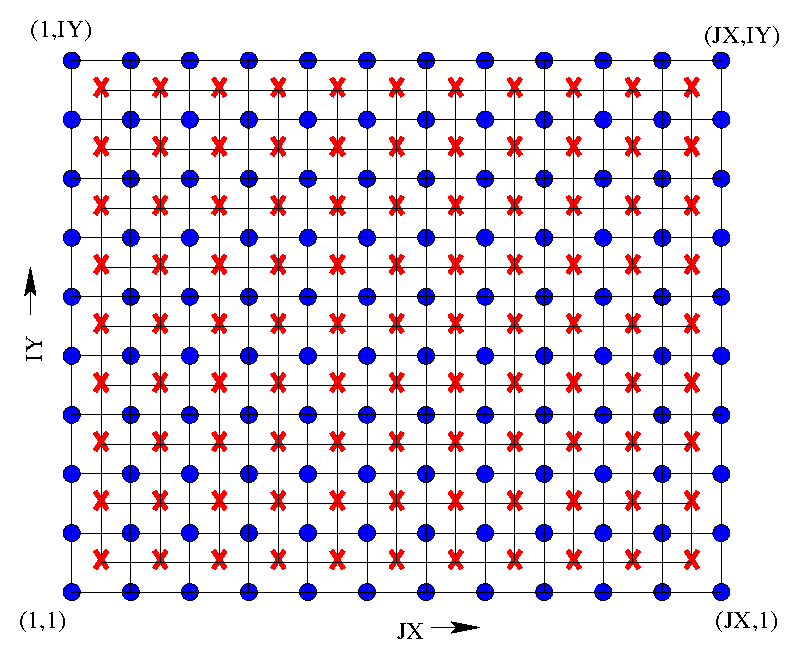
\includegraphics{mm5_grid2.eps}}
\caption{Schematic representation showing the horizontal Arakawa B-grid
staggering of the dot ($U,V$) and cross ($T,Q,\dots$) grid points.}
\label{mm5_grid}
\end{center}
\end{figure}

\begin{figure}
\begin{center}
\resizebox{3.7in}{!}{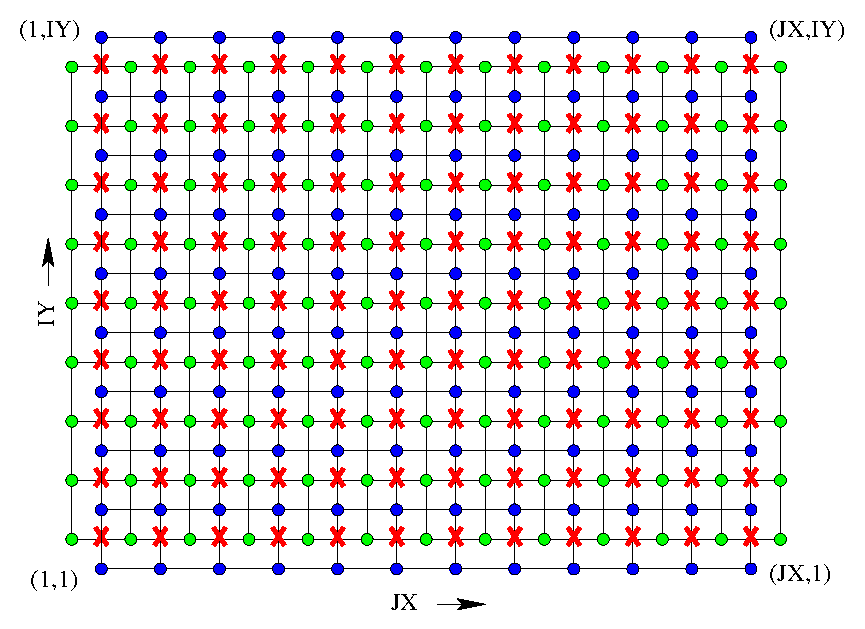
\includegraphics{moloch_grid2.eps}}
\caption{Schematic representation showing the horizontal Arakawa C-grid
staggering of the dot-$U$ (green), dot-$V$ (blue) and cross ($T,Q,\dots$)
grid points.}
\label{mo_grid}
\end{center}
\end{figure}

\section{The \ac{RegCM} Model Vertical Grid}

All the status variables are defined in the middle of each model vertical layer,
referred to as half-levels and represented by the dashed lines in
Figure~\ref{sigma_levels}. Vertical velocity is carried instead at the full
levels (solid lines).

In defining the sigma levels it is the full levels that are
listed, including levels at $\sigma$ = 0 and 1. The number of model layers is
therefore always one less than the number of full sigma levels.

\subsection{Pressure based Vertical Coordinates}

\begin{figure}
\begin{center}
\resizebox{3.5in}{!}
{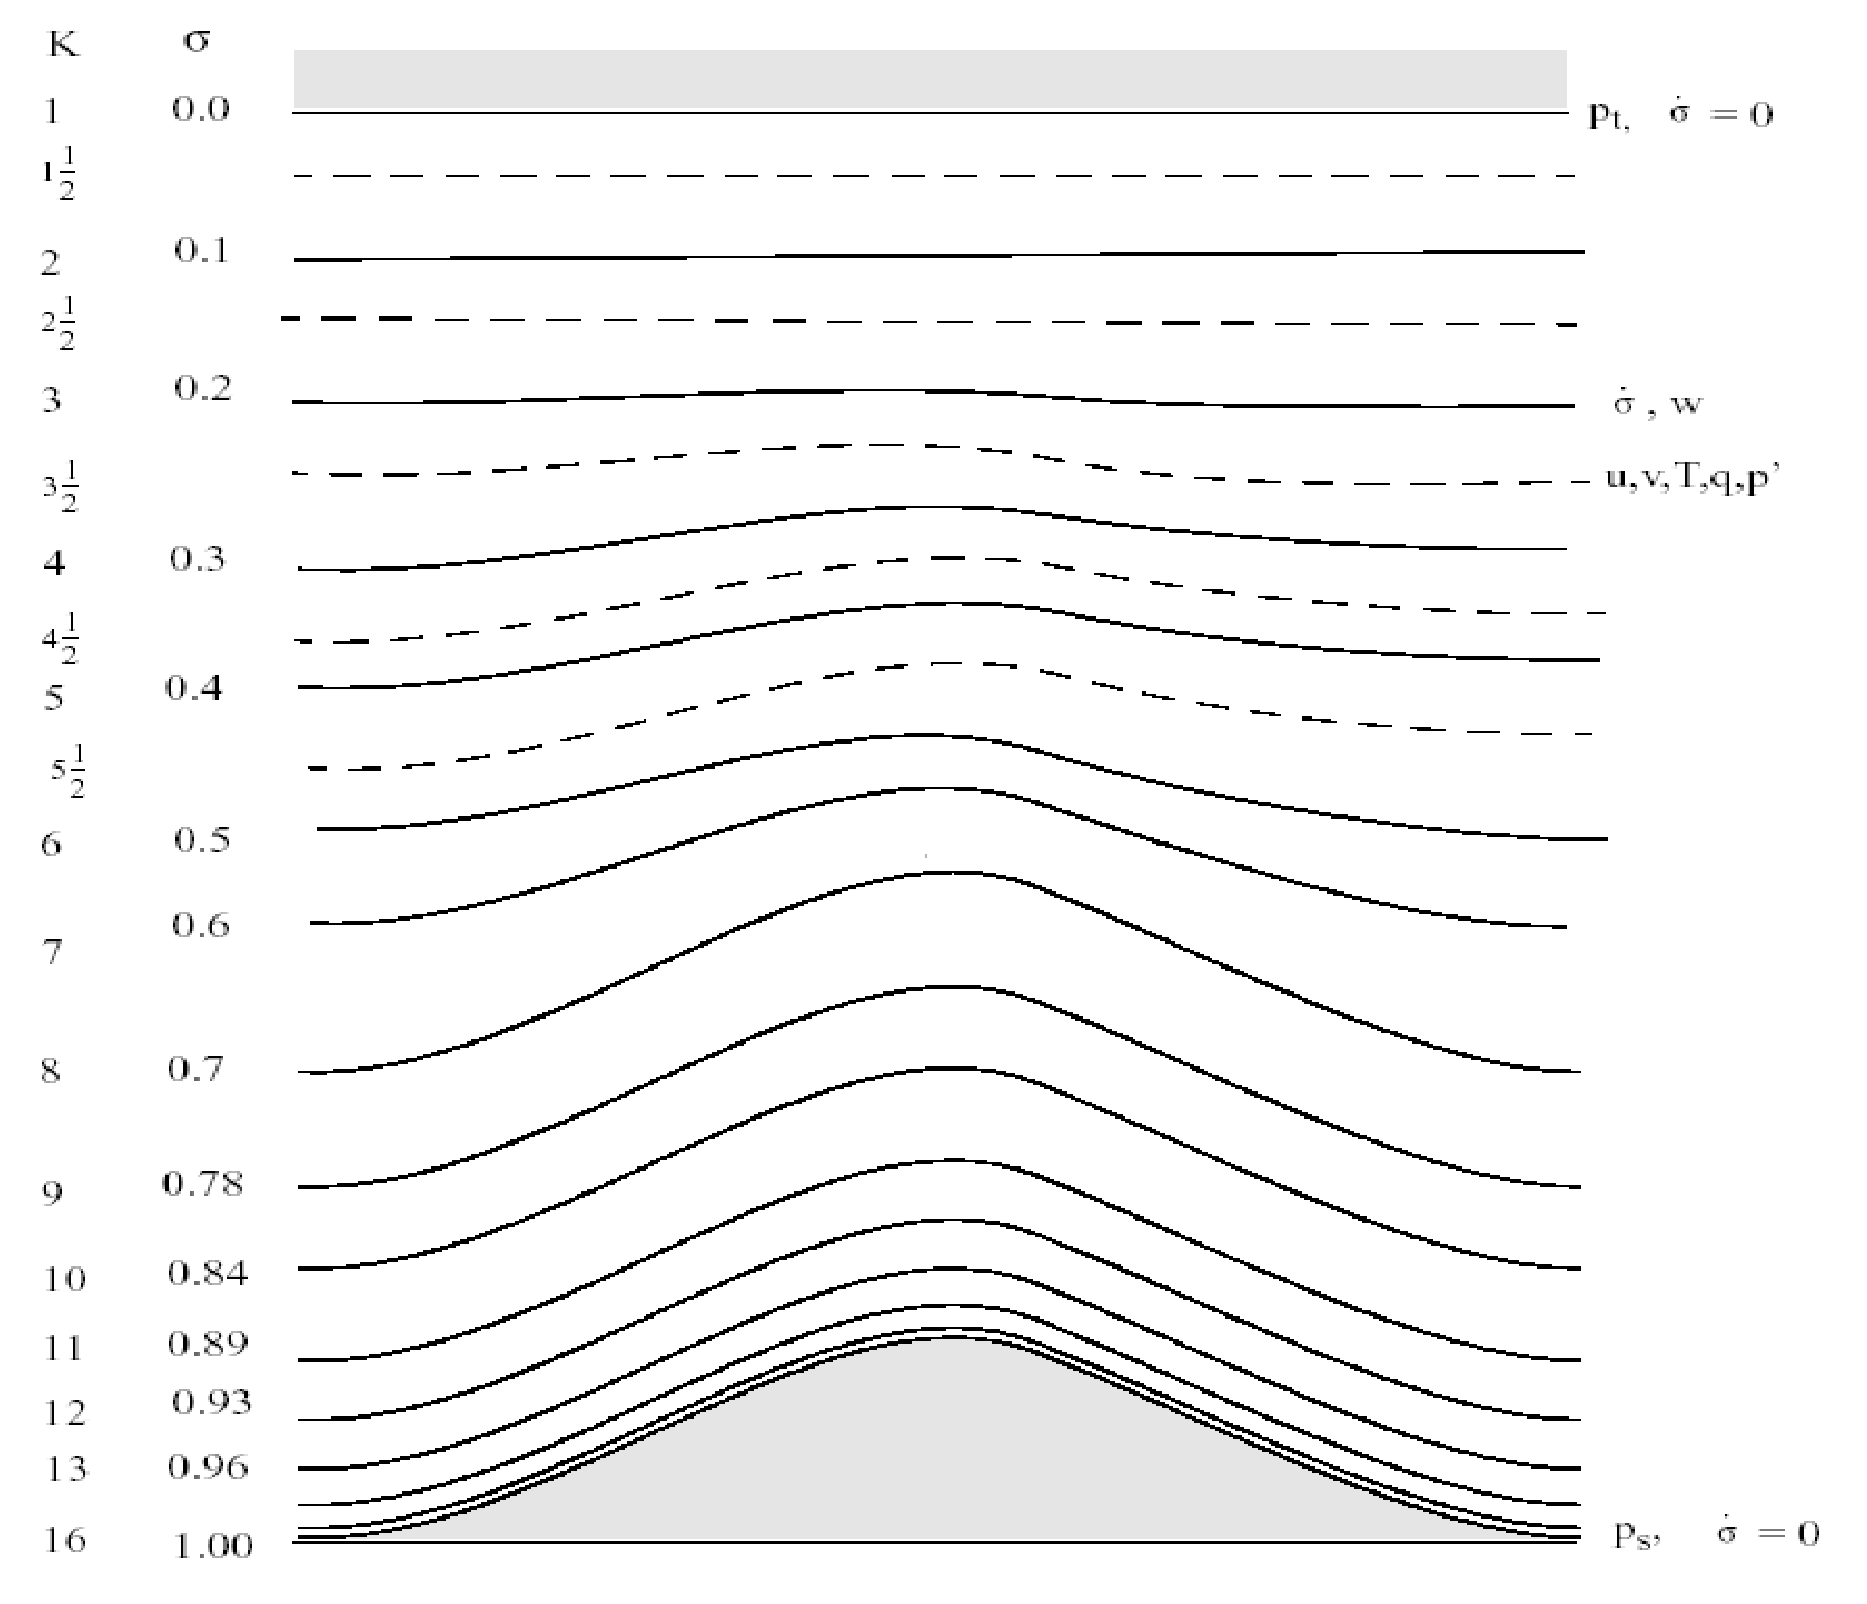
\includegraphics{sigma_levels.eps}}
\caption{Schematic representation of the vertical structure of the pressure
based levels of the model.
This example is for $KZ$ vertical layers. Dashed lines denote full-sigma levels,
solid lines denote half-sigma levels.}
\label{sigma_levels}
\end{center}
\end{figure}

The vertical coordinate for the \ac{MM5} derived dynamical cores are
terrain-following (Figure~\ref{sigma_levels}) pressure, meaning
that the lower grid levels follow the terrain, while the topmost surface is
flat with user imposed configurable top rigid lid pressure.
Intermediate levels progressively flatten as the pressure decreases
toward the top of the model. 

The Hydrostatic solver uses a dimensionless $\sigma$ coordinate to
define the model levels where $p$ is the pressure, $p_t$ is a specified
constant top pressure, $p_s$ is the surface pressure.

\begin{eqnarray}
  \sigma = {(p - p_t) \over (p_s - p_t)}
\end{eqnarray}

where we can define:

\begin{eqnarray}
  p^*(x,y) = p_s(x,y) - p_t
\end{eqnarray}

For the Non-hydrostatic solver, a similar dimensionless coordinate is used,
but it is defined entirely from the reference pressure. Given a reference
atmospheric profile:

\begin{eqnarray}
  p(x,y,z,t) = p_0(z) + p^\prime(x,y,z,t) \\
  T(x,y,z,t) = T_0(z) + T^\prime(x,y,z,t) \\
  \rho(x,y,z,t) = \rho_0(z) + \rho^\prime(x,y,z,t)
\end{eqnarray}

the vertical sigma coordinate is defined as:

\begin{eqnarray}
  \sigma = {(p_0 - p_t) \over (p_s - p_t)}
\end{eqnarray}

where $p_s$ is the surface pressure, $p_t$ is a specified constant top
pressure and $p_0$ is the reference pressure profile. The total pressure
at each grid point is thus given as:

\begin{eqnarray}
 p = p^*\sigma + p_t + p^\prime
\end{eqnarray}

with $p^*$ defined as in the hydrostatic solver.

It can be seen from the equation and Figure~\ref{sigma_levels} that $\sigma$ is
zero at the top and one at the surface, and each model level is defined by a
value of $\sigma$. The model vertical resolution is defined by a list of values
between zero and one that do not necessarily have to be evenly spaced. Commonly
the resolution in the boundary layer is much finer than above, and the number of
levels may vary upon the user demand.

\subsection{$H$ based Vertical Coordinate}
\label{h_coordinate}

\begin{figure}
\begin{center}
\resizebox{3.5in}{!}
{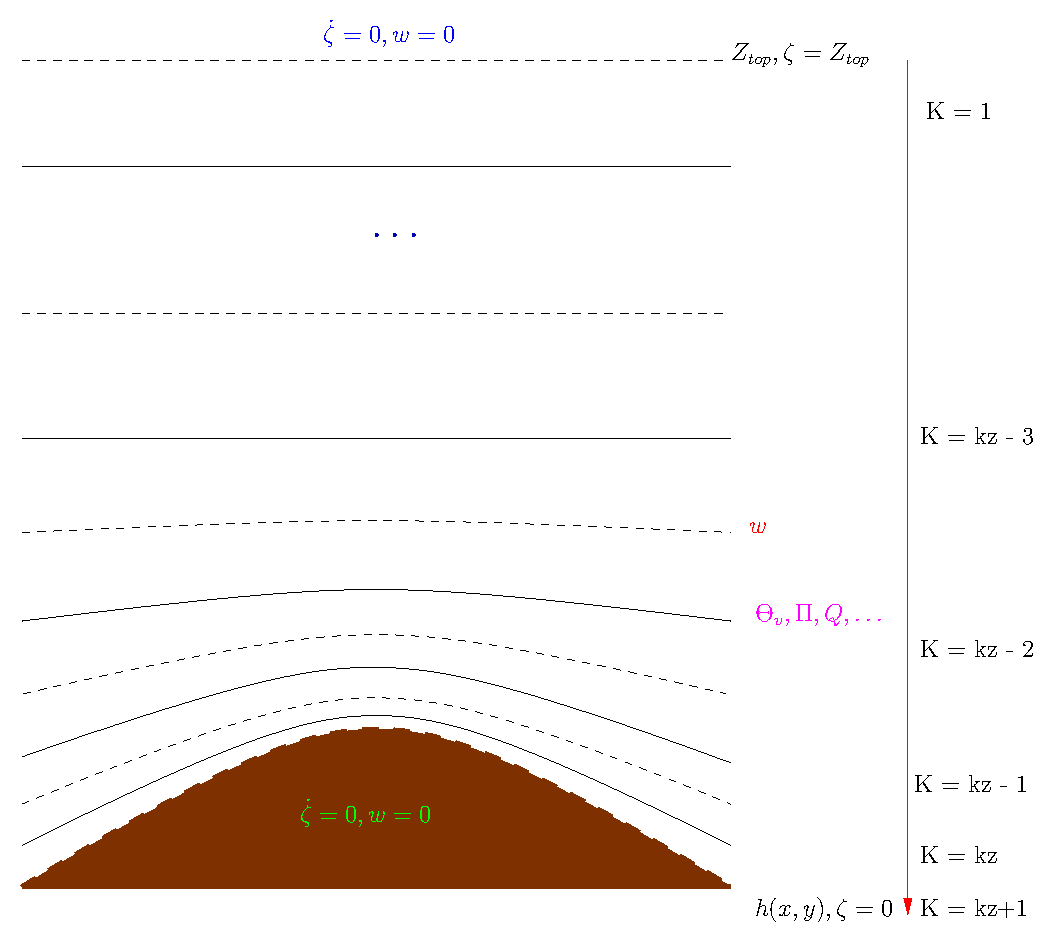
\includegraphics{moloch_levels.eps}}
\caption{Schematic representation of the vertical structure of the $H$
based levels of the model.
This example is for $KZ$ vertical layers. Dashed lines denote full-sigma levels,
solid lines denote half-sigma levels.}
\label{moloch_levels}
\end{center}
\end{figure}

The \ac{MOLOCH} dynamical core uses a terrain following $H$ coordinate
$\zeta$ (Figure~\ref{moloch_levels}) which transform the semi-infinite z
interval $[h, \infty)$ into the finite interval $[0,H]$ and is defined as:

\begin{equation}
\zeta = H \left( 1 - e^{-\frac{z - G(\zeta)h(x,y)}{B(\zeta) H}} \right)
\end{equation}

where $h(x,y)$ is the local topography and $G(\zeta)$ and $B(\zeta)$ have the
following analythical formulation:

\begin{eqnarray}
G(\zeta) &=& 1 - a_0 \frac{\zeta}{H} -
       (3 - 2 a_0)\left( \frac{\zeta}{H} \right)^2 +
       (2 - a_0) \left( \frac{\zeta}{H} \right)^3 \\
B(\zeta) &=& b_0 + (1-b_0) \frac{\zeta}{H}
\end{eqnarray}

where $H$ is the scale height of the atmosphere defined as function of
reference climatological surface temperature $T_0$ as:

\begin{equation}
H = R_d T_0 / g
\end{equation}

and the $a_0$ and $b_0$ are configurable constant parameters with:

\begin{equation}
0 \le a_0 \le 1 \quad , \quad 0 \le b_0 \le 1
\end{equation}

\section{Map Projections and Map-Scale Factors}
The modeling system has a
choice of four map projections. Lambert Conformal is suitable for mid-latitudes,
Polar Stereographic for high latitudes, Normal Mercator for low latitudes, and
Rotated Mercator for extra choice. The $x$ and $y$ directions in the model do
not correspond to west-east and north-south except for the Normal Mercator
projection, and therefore the observed wind generally has to be rotated to the
model grid, and the model $u$ and $v$ components need to be rotated before
comparison with observations. These transformations are accounted for in the
model pre-processors that provide data on the model grid (Please note that
model output of u and v components, raw or postprocessed, should be rotated to a
lat/lon grid before comparing to observations).  The map scale factor, $m$, is
defined by:

\begin{equation}
  m = \frac{model\_grid\_distance}{real\_earth\_distance}
\end{equation}

\noindent \\ and its value is usually close to one, varying with latitude. The
projections in the model preserve the shape of small areas, so that $dx=dy$
everywhere, but the grid length varies across the domain to allow a
representation of a spherical surface on a plane surface. Map-scale factors need
to be accounted for in the model equations wherever horizontal gradients are
used.

